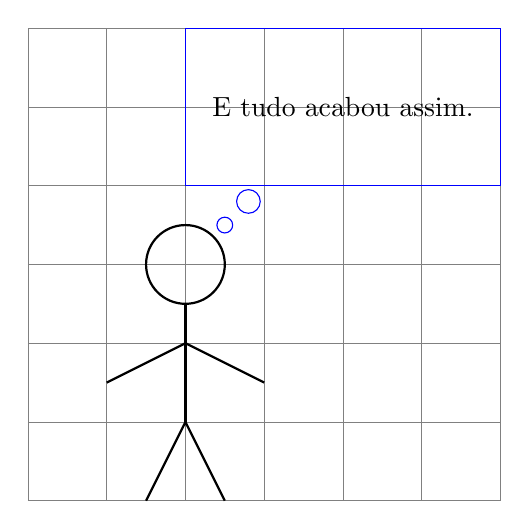
\begin{tikzpicture}
\draw[help lines] (0,0) grid (6,6);
\draw[thick] (2,3) circle (0.5);
\draw[thick] (2,2.5) -- (2,1);              % corpo
\draw[thick] (1,1.5) -- (2,2) -- (3,1.5);   % braços
\draw[thick] (1.5, 0) -- (2,1) -- (2.5, 0); % pernas
\draw[blue] (2,4) rectangle (6,6);
\draw[blue] (2.5,3.5) circle (0.1);
\draw[blue] (2.8,3.8) circle (0.15);
\node at (4,5) {E tudo acabou assim.};
\end{tikzpicture}
